%!TEX root = ../../main.tex
\section{Applying the RDE to DWD}
\label{sec:Applying the RDE to DWD}
\textcolor{red}{
    \begin{myenumerate}
        \item \hypertarget{todo:change section name}{\textbf{TODO:}This section name doesn't sound great either.}
    \end{myenumerate}
}
The RDE is a monotonically decreasing function of the dose which is bounded between the values of 0 and 1 (equation \ref{eqrdeleal}).
If $\eta = \text{RDE}$ then the decreasing nature of the RDE means that as the dose increases the DWD defined in equation \ref{eq:DWD equation with RDE} will decrease at some point.
This may be a desirable characteristic if only diffraction is to be considered.
However if the DWD is used to characterise the damage in a crystal, then it would be expected to always increase with increasing radiation exposure.
For this reason two forms of $\eta$ were investigated.
\begin{align}
    \eta &= \text{RDE}, \label{eq:Decreasing eta form} \\
    \eta &= 1 - \text{RDE}. \label{eq:Increasing eta form}
\end{align}
Both forms are bounded between 0 and 1.
The difference between them is that equation \ref{eq:Decreasing eta form} decreases from 1 to 0 whereas equation \ref{eq:Increasing eta form} increases from 0 to 1 Figure~\ref{fig:Different Eta forms}.
\begin{figure}
        \centering
        \begin{subfigure}[b]{0.45\textwidth}
                \centering
                \includegraphics[width=\textwidth]{figures/dwd/EtaDecreasing.pdf}
                \caption{}
                \label{fig:Decreasing Eta}
        \end{subfigure}
			\quad
        \begin{subfigure}[b]{0.45\textwidth}
                \centering
                \includegraphics[width=\textwidth]{figures/dwd/EtaIncreasing.pdf}
                \caption{}
                \label{fig:Increasing Eta}
        \end{subfigure}
        \caption{Two different forms of $\eta$ used in equation \ref{eq:DWD equation with RDE}. (a) $\eta = \text{RDE}$. (b) $\eta = 1-\text{RDE}$.}
        \label{fig:Different Eta forms}
\end{figure}

The remainder of this section presents the results of the analysis carried out with the data from \cite{zeldin2013dwd} using the forms of $\eta$ given above, comparing their performance with the simple DWD (equation \ref{eq:DWD equation - no RDE}).

\subsection{Predicting intensity loss}
\label{sub:Predicting intensity loss}
In the study carried out by Zeldin \textit{et al.} \cite{zeldin2013dwd} cubic crystals of bovine pancreatic insulin were irradiated under different dose contrast conditions.
The three beams used in the study: big, medium and small, are shown in Figure~\ref{fig:Big, medium and small beams - Oli experiment}.
\begin{figure}
  \centering
    \includegraphics[width=1\textwidth]{figures/dwd/Oli_beams.png}
    \caption{False color images of the beam profiles used for the experiments in \cite{zeldin2013dwd}. The pixel size is $\text{5} \times \text{5}\,\mu m^2$ in all cases. (a) Big beam. (b) Medium beam. (c) Small beam.}
    \label{fig:Big, medium and small beams - Oli experiment}
\end{figure}
It was shown that the DWD is a significantly better metric for assessing the extent of radiation damage compared to the average dose for the whole crystal (AD-WC) or the maximum dose, because the spread of relative intensity values was greatly reduced.
The data for the big and small beams were available so the same relative intensity data were generated using the different $\eta$ forms.
The results are shown in Figure~\ref{fig:Relative intensity - DWD eta forms}.
The main difference that can be seen from the plots is the DWD range.
The increasing $\eta$ function results in the largest range of DWD values.
Conversely, the decreasing $\eta$ function reduces the range of DWD values.
Another difference is that introducing the $\eta$ function shifts the big beam data relative to the small beam data.
The increasing $\eta$ function shifts the big beam data down, relative to the small beam data, whereas the decreasing $\eta$ function shifts the big beam data down.
This suggests that there is a signature from the different beams.
However this is an undesirable effect because DWD should already account for the different beam conditions via the flux weighting.
\begin{figure}
	\centering
    \begin{subfigure}[b]{1\textwidth}
        \centering
        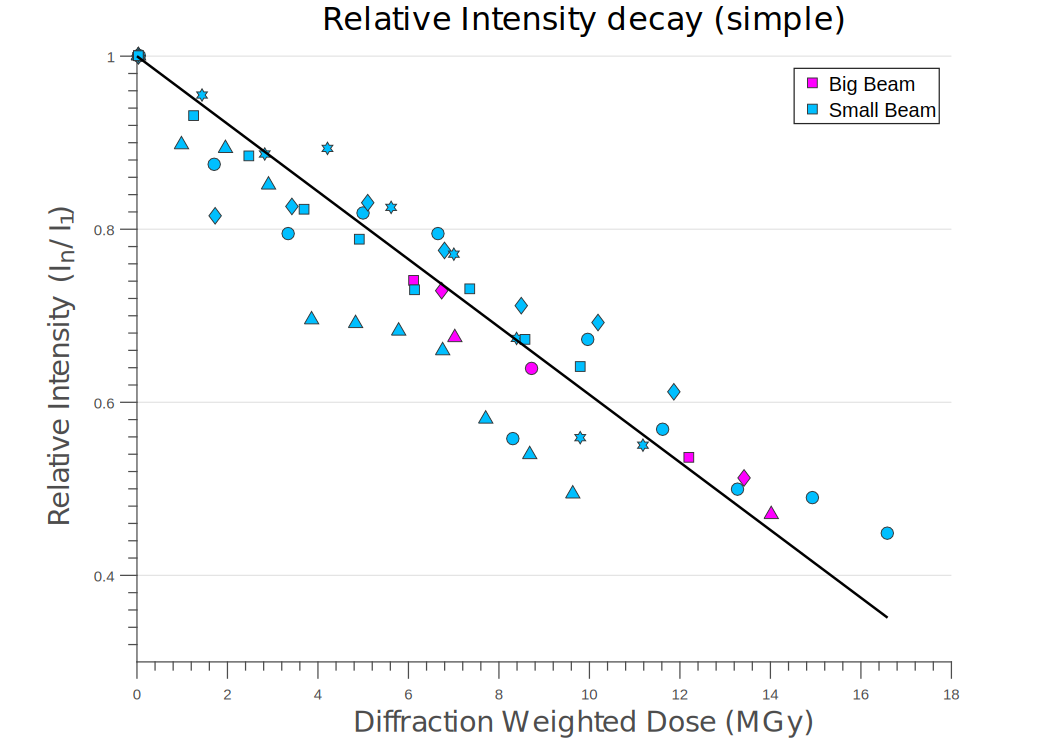
\includegraphics[width=\textwidth]{figures/dwd/reproduce_relint_DWDsimple.pdf}
        \caption{}
        \label{fig:Relative intensity - Simple DWD}
    \end{subfigure}
    \\
	\begin{subfigure}[b]{1\textwidth}
        \centering
        \includegraphics[width=\textwidth]{figures/dwd/reproduce_relint_DWDnew.pdf}
        \caption{}
        \label{fig:Relative intensity - Increasing Eta}
    \end{subfigure}
\end{figure}
\begin{figure}
\ContinuedFloat
    \begin{subfigure}[b]{1\textwidth}
        \centering
        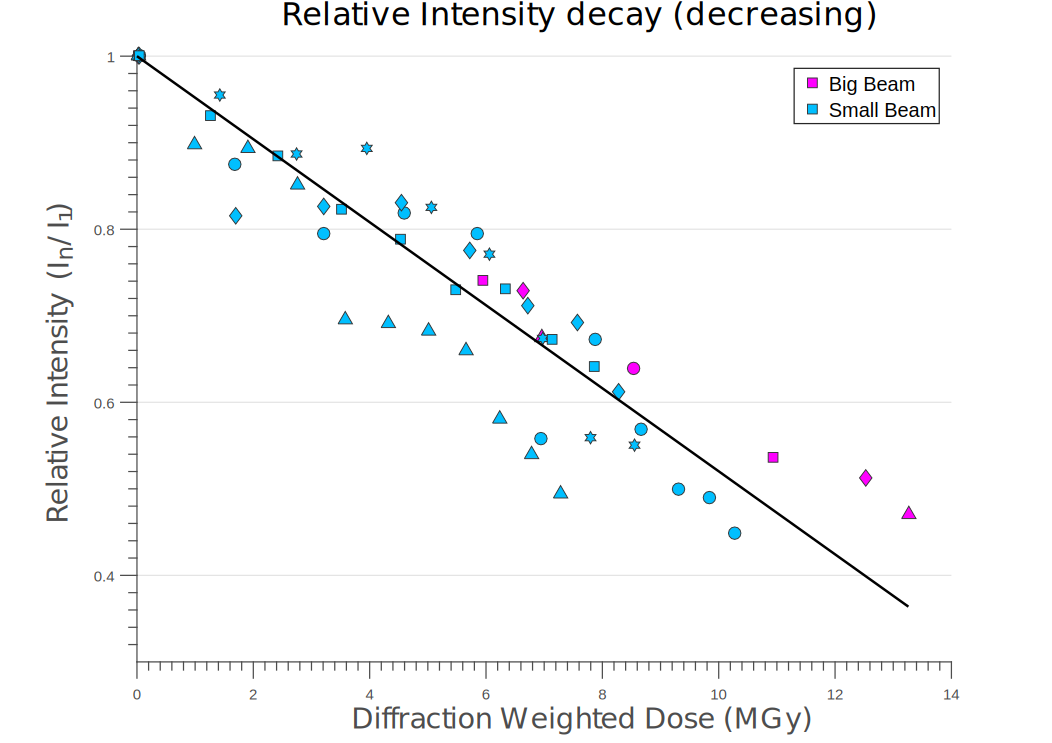
\includegraphics[width=\textwidth]{figures/dwd/reproduce_relint_DWDwrong.pdf}
        \caption{}
        \label{fig:Relative intensity - Decreasing Eta}
    \end{subfigure}
	\caption{}
	\label{fig:Relative intensity - DWD eta forms}
\end{figure}

A line of best fit was calculated using a least squares fitting procedure and plotted (solid black line Figure~\ref{fig:Relative intensity - DWD eta forms}).
A measure of the overall deviation of the data from the line was obtained by calculating the squared Euclidean norm\footnote{The squared Euclidean norm is defined as $\sum_i (f(x_i) - y_i)^2$} for each DWD form (Table~\ref{tab:Squared Euclidean norm values - Relative intensity fits}).
The DWD form that gave the lowest value for the squared Euclidean norm was the simple DWD form.
This suggests that the data are less spread overall without adding a functional form for $\eta$.
\begin{table}[ht!]
\small
\captionsetup{justification=centering}
	\caption{Squared Euclidean norm values of the line of best fit with the data in Figure~\ref{fig:Relative intensity - DWD eta forms}.}
	\centering
	\begin{tabular}{p{5cm} p{4.5cm}}
		$\eta$ form			                & Squared Euclidean norm    \\
		\hline
		$\eta = 1$ (simple)     			& 0.2034        \\
		$\eta = RDE$ (decreasing)     	    & 0.2112        \\
		$\eta = 1-RDE$ (increasing)    		& 0.2060       \\
		\hline
	\end{tabular}
	\label{tab:Squared Euclidean norm values - Relative intensity fits}
\end{table}

$D_{1/2}$ is a metric of the radiation sensitivity of a protein crystal that is defined as the dose at which the relative intensity falls to 50\%.
$D_{1/2}$ values were calculated from the line of best fit for each of the DWD forms.
Furthermore $s_{AD}$ values were also calculated and both sets of values are given in Table~\ref{tab:Half dose and SAD values}.
\begin{table}[ht!]
\small
\captionsetup{justification=centering}
	\caption{Parameter values for Leal \emph{et al.} model determined by the method described in section \ref{sub:Obtaining Model Parameter Values} with data scaled to different resolution limits.}
	\centering
	\begin{tabular}{p{2cm}*{6}{c}r}
	\cline{2-4} \cline{5-7}
		& \multicolumn{3}{c}{$D_{1/2}$ (MGy)} & \multicolumn{3}{c}{$s_{AD}$ (\AA$^2$/MGy)} \\
		\cmidrule(l{2pt}r{2pt}){2-4} \cmidrule(l{2pt}r{2pt}){5-7}
		Beam size			&Simple	    &Decreasing   &Increasing     &Simple	    &Decreasing   &Increasing	\\
		\hline
		Big beam    		&12.94	    &12.18 	      &13.97         &0.0125	    &0.0133	      &0.0116	\\
		Small beam     		&13.32		&9.91 	      &17.84         &0.0068	    &0.0092       &0.0050     \\
		\hline
	\end{tabular}
	\label{tab:Half dose and SAD values}
\end{table}
The spread of the $D_{1/2}$ values for the simple DWD, $0.38\,$MGy, is much smaller than the spread for the decreasing $\eta$ form, $2.27\,$MGy, and the increasing $\eta$ form, $3.87\,$MGy.
This confirms the result that the spread of the data is increased by incorporating the dose dependent $\eta$ forms.
The ranges of $s_{AD}$ values are not greatly improved by adding the dose dependent forms of $\eta$ to the DWD equation.
However, given the fact that DWD does not significantly reduce the data spread for the $B_{rel}$ metric \cite{zeldin2013dwd}, a reduction in the spread of $s_{AD}$ values was not expected.

\subsection{Offset Simulations}
\label{sub:Offset Simulations}
Zeldin \textit{et al.} defined the diffracted dose efficiency (DDE) as the ratio of elastically scattered photons to DWD as a measure of the efficiency of a given data collection strategy.
The DDE states the number of elastically scattered photons that are diffracted per unit dose and it is this quantity that is to be maximised for a given experiment.
To test this, the authors simulated experiments where the rotation axis was offset from the beam axis by various distances to see how spreading the dose changed the DDE.
These simulations were performed for each of the DWD forms.  
